\subsection{Input resolution vs.\ architecture}
\label{sec:res}
\ifHaveResSweep
The comparison above pits \yolo{} at 1280\,px against \rfdetr{} at 640\,px (its native Nano resolution is 384\,px).
Fig.~\ref{fig:res} re-scores every model at six input sizes (no retraining), and \yolo{} is additionally fine-tuned
at 640\,px (\emph{FT@640}, 80-class head, otherwise the same recipe). \emph{At matched input size the in-domain
gap disappears.} Trained and tested at 640\,px, \yolo{} reaches \AP{}~\MsRsixAa{} against \MsRfFtAa{} for \rfdetr; tested at
1280\,px the fine-tuned students tie in-domain (\RsFteFAa{} vs.\ \RsRfFtFAa) but \rfdetr{} generalises far better to
the held-out video at every size (\RsRfFtFHo{} vs.\ \RsFteFHo{} at 1280\,px, the best held-out score of any model in
this study). The in-domain advantage of \yolo{} in Table~\ref{tab:det} is therefore a resolution effect, not an
architecture effect. What \yolo{} does buy is compute: \CsYFGf{} GFLOPs at $736{\times}1280$ against \CsRCGf{} for
\rfdetr{} at $640{\times}640$ and \CsRFGf{} at $1280{\times}1280$ (\CsRatioF$\times$). At the closest compute
(\rfdetr{} at 384\,px, \CsRAGf{} GFLOPs, still more than \yolo{} at 1280\,px) \yolo{} is far better in-domain (\RsFteFAa{} vs.\
\RsRfFtAAa) and similar on the held-out video (\RsFteFHo{} vs.\ \RsRfFtAHo). The COCO-pretrained \rfdetr{} likewise
improves from \RsRfPtAAa{} at its native 384\,px to \RsRfPtEAa{} at 960\,px, so the weak pretrained baseline of
Table~\ref{tab:det} reflects its input size too.
\ifHaveCostLat Measured on the desktop GPU, the deployed paths take \CsYFLat\,ms (\yolo{}, 1280) and \CsRCLat\,ms /
\CsRFLat\,ms (\rfdetr{}, 640 / 1280) per frame.\fi

\figif{fig_resolution.pdf}{%
\begin{figure*}[t]
\centering
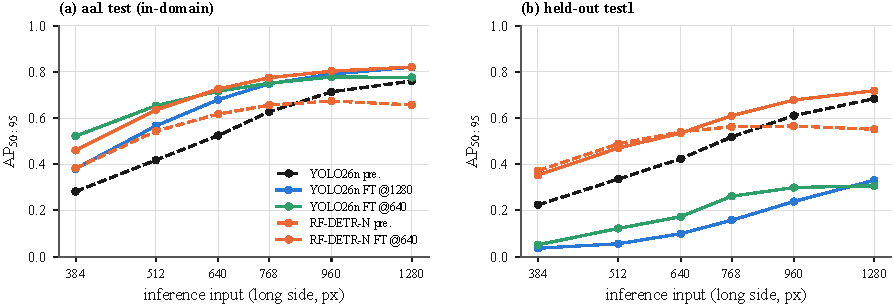
\includegraphics[width=\textwidth]{figures/fig_resolution.pdf}
\caption{\AP{} vs.\ inference input size, without retraining (``FT @640'' was trained at 640\,px, all other
fine-tuned models at their deployment size). (a)~aa1 test; (b)~held-out test1. At equal input size \rfdetr{}
matches \yolo{} in-domain and is far more robust on the held-out video, at 25--44$\times$ the GFLOPs of \yolo{} at the
same input size.}
\label{fig:res}
\end{figure*}}
\else
The resolution-matched comparison is pending.
\fi
